\lecture{2}{22/1}
\section{Flow}

We have a common scenario where material transferred from a
\emph{source} to a \emph{sink}.
The source produces at a steady rate, as does the sink consuming.

\begin{example}
    Examples of real world flow problems:
    \begin{enumerate}
        \item water through pipes;
        \item current through circuit;
        \item data through network; and
        \item trucks from factory to warehouse. 
    \end{enumerate}
\end{example}

We can use graphs to represent these problems where edges have a given
\emph{capacity} and vertices are \emph{junctions}.
The flow into a vertex must equal the flow going out,
but we will see this formally later.

\begin{problem}[Maximum flow problem]
    What is the greatest rate of transportation from source to sink?
\end{problem}

Our flow network $G = (V,E)$ is a directed graph with two distinct
$s, n \in V$. 
We have a capacity function $c: V \times V \to \R$ where
$c(u, v) \geq 0$ if $(u, v) \in E$ and
$c(u, v) = 0$ if $(u,v) \not\in E$.
We assume that all vertices lie on a path between $s$ and $t$
and so $G$ is connected and $\lvert E \rvert \geq \lvert V \rvert - 1$.

\begin{definition}[Flow constraints]
    A \textbf{flow} in a flow network $G = (V, E)$
    is a function $f: V \times V \to \R$
    that satisfies
    \begin{enumerate}
        \item (capacity constraint) for all $u,v \in V: f(u,v) \leq c(u,v)$;
        \item (skew symmetry) for all $u,v \in V: f(u,v) = -f(v,u)$; and
        \item (flow conservation) for all $u \in V \setminus \{s, t\}: \sum_{v \in V} f(u,v) = 0$.
    \end{enumerate}
\end{definition}

\begin{definition}[]
    Let $G = (V, E)$ be a flow network.
    The \textbf{total positive flow entering} $v \in V$ is
    \[ 
        x_e(v) = \sum_{u \in V: f(u,v) > 0} f(u,v) 
    \]
    and the \textbf{total positive flow leaving} $u \in V$ is
    \[ 
        x_l(u) = \sum_{v \in V: f(u,v) > 0} f(u,v). 
    \]
    The \textbf{total net flow} $x$ at a vertex $v$ is defined as
    \[ 
        x(v) = x_e(v) - x_l(v). 
    \]
\end{definition}

\begin{definition}[Flow value]
    Let $G = (V, E)$ be a flow network and let $f$ be a flow in $G$.
    The \textbf{value} of flow is the total flow leaving the source
    \[
        \lvert f \rvert = \sum_{v \in V} f(s, v).
    \]
\end{definition}

Note that the notation used here \emph{does not} mean absolute.

\begin{proposition}
    Let $G  = (V, E)$ and $X, Y, Z \subset V$.
    Then
    \begin{enumerate}
        \item
            \[
                f(X, Y) = \sum_{x \in X} \sum_{y \in Y} f(x, y);
            \]
            
        \item
            \[
                f(X, X) = 0;
            \]
            
        \item
            \[
                f(X, Y) = -f(Y, X);
            \]
            
        \item if $X \cap Y = \varnothing$
            \begin{align*}
                f(X \cup Y, Z) &= f(X, Z) + f(Y, Z) \\
                f(Z, X \cup Y) &= f(Z, X) + f(Z, Y).
            \end{align*}
    \end{enumerate}
\end{proposition}

We will now introduce a the \emph{Ford-Fulkerson method},
a greedy algorithm that computes the maximum flow in a flow network.
The general idea is to construct residual networks consisting
of edges that can admit more flow.

More formally, consider $u, v \in V$ for a flow network $G = (V, E)$.
The amount of additional flow we can push from $u$ to $v$ before
exceeding $c(u, v)$ is the residual capacity of $(u, v)$. That is,
\[
    c_f(u,v) = c(u,v) - f(u,v).
\]

\begin{remark}
    If $f(u,v) < 0$, then $c_f(u,v) > c(u,v)$.
    That is, we cannot expect residuals capacities to be bounded above
    by the capacity of the edge if we have negative flows.
\end{remark}

\begin{lemma}
    Let $G = (V, E)$ be a flow network, $f$ be a flow in $G$,
    $G_f$ be the residual network of $G$ \emph{induced by} $f$,
    and let $f'$ be a flow in $G_f$.
    Then the flow sum $f + f'$ defined by
    \[
        (f + f')(u,v) = f(u,v) + f'(u,v)
    \]
    is a flow in $G$ with value 
    $\lvert f+f' \rvert = \lvert f \rvert + \lvert f' \rvert$.
\end{lemma}

\begin{definition}
    Let $G = (V, E)$ be a flow network and $f$ be a flow in $G$.
    Then a simple path $P \subset E$ in $G_f$ is \textbf{augmenting}.
\end{definition}

We can then increase the flow along an augmenting path $P$ by
\[
    c_f(P) = \min_{(u,v) \in P} c_f(u,v).
\]

\begin{lemma}[]
    Let $G = (V,E)$ be a flow network,
    $f$ be a flow in $G$,
    and let $P$ be an augmenting path in $G_f$.
    We define $f_P$ by
    \[
        f_P(u,v) =
        \begin{cases}
            c_f(P)  & (u,v) \in P \\
            -c_f(P) & (v,u) \in P \\
            0       & \text{otherwise}.
        \end{cases}
    \]
    $f_p$ is a flow in $G_f$ with value $\abs{f_p} = c_f(P) > 0$.
\end{lemma}

\begin{corollary}
    Let $G = (V,E)$ be a flow network,
    $f$ be a flow in $G$,
    $P$ be an augmenting path in $G_f$,
    and $f_P$ be defined as in the previous lemma.
    We define $f' = f + f_P$.
    Then $f'$ is a flow in $G$ with value
    $\abs{f'} = \abs f + \abs{f_P} > \abs f$.
\end{corollary}

\begin{algorithm}
    \hfill
    \begin{algorithmic}
        \Procedure{Ford-Fulkerson}{$G, s, t$}
            \For{$(u,v) \in E$}
                \State $f(u,v) \gets 0$
                \State $f(u,v) \gets 0$
            \EndFor
            \While{$\;\exists\; P = s \to t \in G_f$}
                \State $c_f(P) \gets \min\{c_f(u,v) : (u,v) \in P\}$
                \For{$(u,v) \in P$}
                    \State $f(u,v) \gets f(u,v) + c_f(P)$ 
                    \State $f(v,u) \gets -f(u,v)$
                \EndFor
            \EndWhile
        \EndProcedure
    \end{algorithmic}
\end{algorithm}

We see that the Ford-Fulkerson algorithm does not specify \emph{how}
to find an augmenting $P \subset G$.

\begin{example}
    Consider the following residual network.
    \begin{center}
        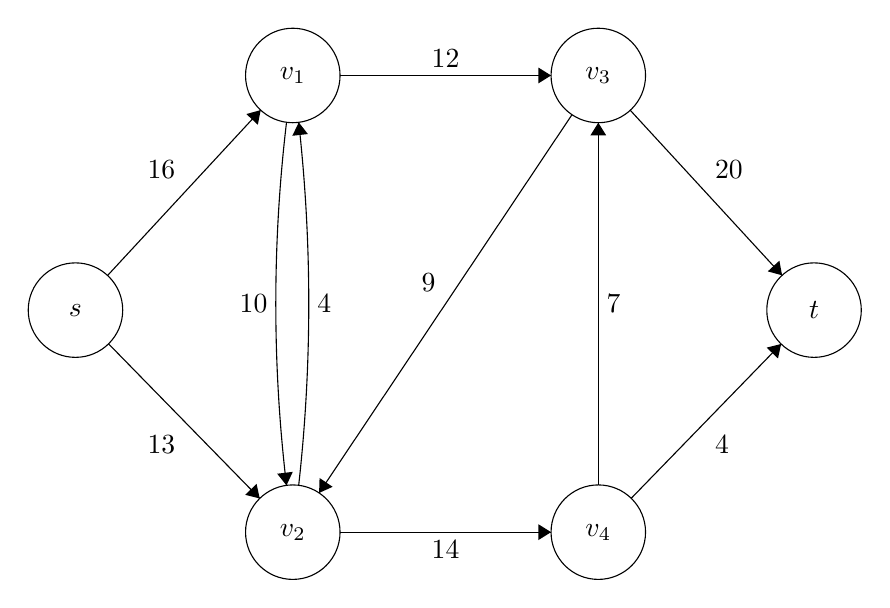
\begin{tikzpicture}[scale=0.2]
            \tikzstyle{every node}+=[inner sep=0pt]
            \draw [black] (5.1,-26) circle (3);
            \draw (5.1,-26) node {$s$};
            \draw [black] (18.9,-11.1) circle (3);
            \draw (18.9,-11.1) node {$v_1$};
            \draw [black] (18.9,-40.1) circle (3);
            \draw (18.9,-40.1) node {$v_2$};
            \draw [black] (38.3,-11.1) circle (3);
            \draw (38.3,-11.1) node {$v_3$};
            \draw [black] (38.3,-40.1) circle (3);
            \draw (38.3,-40.1) node {$v_4$};
            \draw [black] (52,-26) circle (3);
            \draw (52,-26) node {$t$};
            \draw [black] (7.14,-23.8) -- (16.86,-13.3);
            \fill [black] (16.86,-13.3) -- (15.95,-13.55) -- (16.68,-14.23);
            \draw (11.47,-17.09) node [left] {$16$};
            \draw [black] (21.9,-11.1) -- (35.3,-11.1);
            \fill [black] (35.3,-11.1) -- (34.5,-10.6) -- (34.5,-11.6);
            \draw (28.6,-10.6) node [above] {$12$};
            \draw [black] (40.33,-13.31) -- (49.97,-23.79);
            \fill [black] (49.97,-23.79) -- (49.8,-22.86) -- (49.06,-23.54);
            \draw (45.68,-17.09) node [right] {$20$};
            \draw [black] (40.39,-37.95) -- (49.91,-28.15);
            \fill [black] (49.91,-28.15) -- (48.99,-28.38) -- (49.71,-29.07);
            \draw (45.68,-34.52) node [right] {$4$};
            \draw [black] (38.3,-37.1) -- (38.3,-14.1);
            \fill [black] (38.3,-14.1) -- (37.8,-14.9) -- (38.8,-14.9);
            \draw (38.8,-25.6) node [right] {$7$};
            \draw [black] (36.63,-13.59) -- (20.57,-37.61);
            \fill [black] (20.57,-37.61) -- (21.43,-37.22) -- (20.6,-36.66);
            \draw (27.99,-24.26) node [left] {$9$};
            \draw [black] (21.9,-40.1) -- (35.3,-40.1);
            \fill [black] (35.3,-40.1) -- (34.5,-39.6) -- (34.5,-40.6);
            \draw (28.6,-40.6) node [below] {$14$};
            \draw [black] (18.501,-37.127) arc (-173.22938:-186.77062:97.772);
            \fill [black] (18.5,-37.13) -- (18.9,-36.27) -- (17.91,-36.39);
            \draw (17.32,-25.6) node [left] {$10$};
            \draw [black] (19.275,-14.076) arc (6.36043:-6.36043:104.021);
            \fill [black] (19.28,-14.08) -- (18.87,-14.93) -- (19.86,-14.82);
            \draw (20.42,-25.6) node [right] {$4$};
            \draw [black] (7.2,-28.14) -- (16.8,-37.96);
            \fill [black] (16.8,-37.96) -- (16.6,-37.03) -- (15.88,-37.73);
            \draw (11.47,-34.52) node [left] {$13$};
        \end{tikzpicture}
    \end{center}
    If we pick the path $(s,v_1,v_4,v_2,v_4,t)$ we get the following
    flowing network as a result.
    \begin{center}
        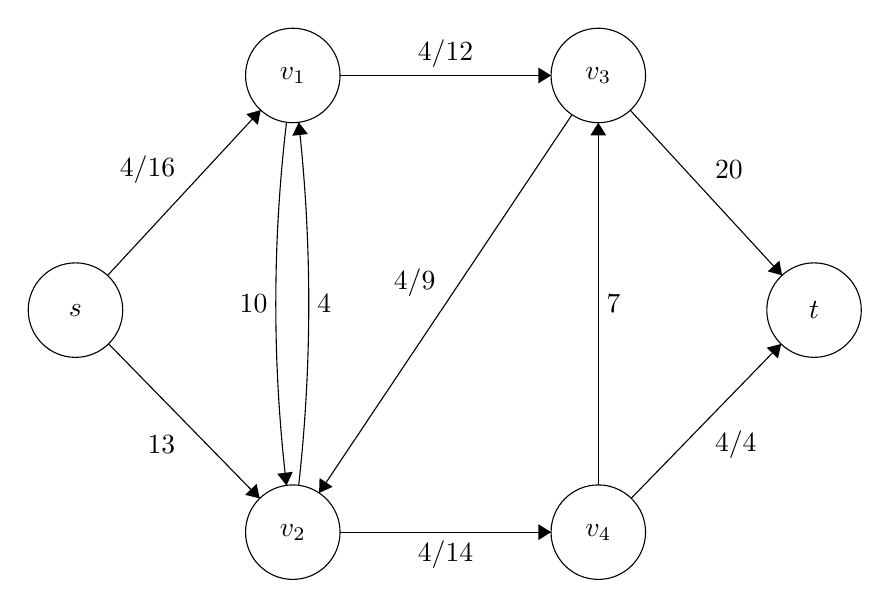
\begin{tikzpicture}[scale=0.2]
            \tikzstyle{every node}+=[inner sep=0pt]
            \draw [black] (5.1,-26) circle (3);
            \draw (5.1,-26) node {$s$};
            \draw [black] (18.9,-11.1) circle (3);
            \draw (18.9,-11.1) node {$v_1$};
            \draw [black] (18.9,-40.1) circle (3);
            \draw (18.9,-40.1) node {$v_2$};
            \draw [black] (38.3,-11.1) circle (3);
            \draw (38.3,-11.1) node {$v_3$};
            \draw [black] (38.3,-40.1) circle (3);
            \draw (38.3,-40.1) node {$v_4$};
            \draw [black] (52,-26) circle (3);
            \draw (52,-26) node {$t$};
            \draw [black] (7.14,-23.8) -- (16.86,-13.3);
            \fill [black] (16.86,-13.3) -- (15.95,-13.55) -- (16.68,-14.23);
            \draw (11.47,-17.09) node [left] {$4/16$};
            \draw [black] (21.9,-11.1) -- (35.3,-11.1);
            \fill [black] (35.3,-11.1) -- (34.5,-10.6) -- (34.5,-11.6);
            \draw (28.6,-10.6) node [above] {$4/12$};
            \draw [black] (40.33,-13.31) -- (49.97,-23.79);
            \fill [black] (49.97,-23.79) -- (49.8,-22.86) -- (49.06,-23.54);
            \draw (45.68,-17.09) node [right] {$20$};
            \draw [black] (40.39,-37.95) -- (49.91,-28.15);
            \fill [black] (49.91,-28.15) -- (48.99,-28.38) -- (49.71,-29.07);
            \draw (45.68,-34.52) node [right] {$4/4$};
            \draw [black] (38.3,-37.1) -- (38.3,-14.1);
            \fill [black] (38.3,-14.1) -- (37.8,-14.9) -- (38.8,-14.9);
            \draw (38.8,-25.6) node [right] {$7$};
            \draw [black] (36.63,-13.59) -- (20.57,-37.61);
            \fill [black] (20.57,-37.61) -- (21.43,-37.22) -- (20.6,-36.66);
            \draw (27.99,-24.26) node [left] {$4/9$};
            \draw [black] (21.9,-40.1) -- (35.3,-40.1);
            \fill [black] (35.3,-40.1) -- (34.5,-39.6) -- (34.5,-40.6);
            \draw (28.6,-40.6) node [below] {$4/14$};
            \draw [black] (18.501,-37.127) arc (-173.22938:-186.77062:97.772);
            \fill [black] (18.5,-37.13) -- (18.9,-36.27) -- (17.91,-36.39);
            \draw (17.32,-25.6) node [left] {$10$};
            \draw [black] (19.275,-14.076) arc (6.36043:-6.36043:104.021);
            \fill [black] (19.28,-14.08) -- (18.87,-14.93) -- (19.86,-14.82);
            \draw (20.42,-25.6) node [right] {$4$};
            \draw [black] (7.2,-28.14) -- (16.8,-37.96);
            \fill [black] (16.8,-37.96) -- (16.6,-37.03) -- (15.88,-37.73);
            \draw (11.47,-34.52) node [left] {$13$};
        \end{tikzpicture}
    \end{center}
    Which results in the following residual network.
        \begin{center}
        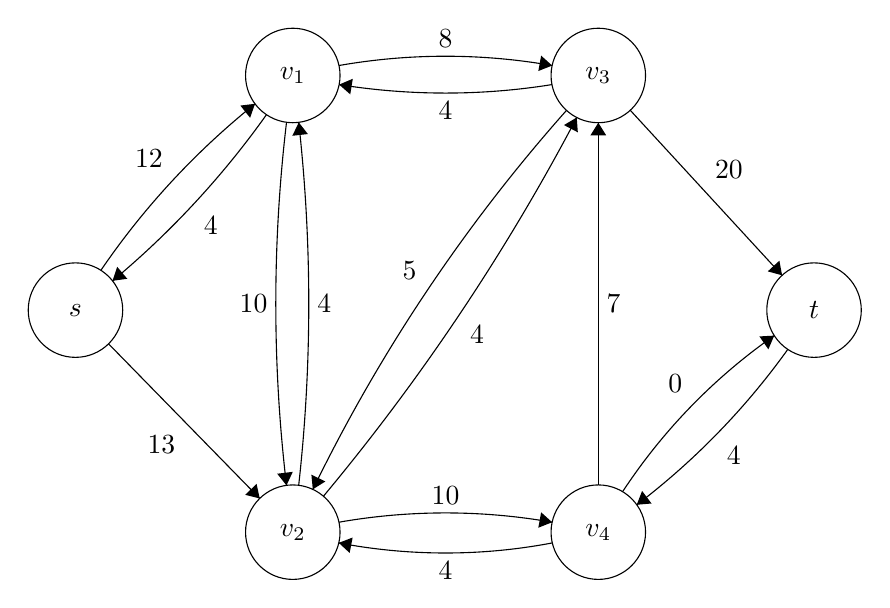
\begin{tikzpicture}[scale=0.2]
            \tikzstyle{every node}+=[inner sep=0pt]
            \draw [black] (5.1,-26) circle (3);
            \draw (5.1,-26) node {$s$};
            \draw [black] (18.9,-11.1) circle (3);
            \draw (18.9,-11.1) node {$v_1$};
            \draw [black] (18.9,-40.1) circle (3);
            \draw (18.9,-40.1) node {$v_2$};
            \draw [black] (38.3,-11.1) circle (3);
            \draw (38.3,-11.1) node {$v_3$};
            \draw [black] (38.3,-40.1) circle (3);
            \draw (38.3,-40.1) node {$v_4$};
            \draw [black] (52,-26) circle (3);
            \draw (52,-26) node {$t$};
            \draw [black] (6.714,-23.472) arc (145.68781:128.70205:48.771);
            \fill [black] (16.5,-12.9) -- (15.57,-13.01) -- (16.19,-13.79);
            \draw (10.68,-16.36) node [left] {$12$};
            \draw [black] (21.832,-10.468) arc (99.96226:80.03774:39.122);
            \fill [black] (35.37,-10.47) -- (34.67,-9.84) -- (34.49,-10.82);
            \draw (28.6,-9.38) node [above] {$8$};
            \draw [black] (40.33,-13.31) -- (49.97,-23.79);
            \fill [black] (49.97,-23.79) -- (49.8,-22.86) -- (49.06,-23.54);
            \draw (45.68,-17.09) node [right] {$20$};
            \draw [black] (39.844,-37.529) arc (146.68286:124.96582:36.68);
            \fill [black] (49.47,-27.62) -- (48.53,-27.67) -- (49.1,-28.49);
            \draw (43.66,-30.64) node [left] {$0$};
            \draw [black] (38.3,-37.1) -- (38.3,-14.1);
            \fill [black] (38.3,-14.1) -- (37.8,-14.9) -- (38.8,-14.9);
            \draw (38.8,-25.6) node [right] {$7$};
            \draw [black] (20.175,-37.384) arc (154.04842:138.38926:106.289);
            \fill [black] (20.17,-37.38) -- (20.97,-36.88) -- (20.08,-36.45);
            \draw (26.79,-23.46) node [left] {$5$};
            \draw [black] (21.832,-39.468) arc (99.96226:80.03774:39.122);
            \fill [black] (35.37,-39.47) -- (34.67,-38.84) -- (34.49,-39.82);
            \draw (28.6,-38.38) node [above] {$10$};
            \draw [black] (18.501,-37.127) arc (-173.22938:-186.77062:97.772);
            \fill [black] (18.5,-37.13) -- (18.9,-36.27) -- (17.91,-36.39);
            \draw (17.32,-25.6) node [left] {$10$};
            \draw [black] (19.275,-14.076) arc (6.36043:-6.36043:104.021);
            \fill [black] (19.28,-14.08) -- (18.87,-14.93) -- (19.86,-14.82);
            \draw (20.42,-25.6) node [right] {$4$};
            \draw [black] (7.2,-28.14) -- (16.8,-37.96);
            \fill [black] (16.8,-37.96) -- (16.6,-37.03) -- (15.88,-37.73);
            \draw (11.47,-34.52) node [left] {$13$};
            \draw [black] (17.228,-13.59) arc (-35.42054:-50.1896:55.95);
            \fill [black] (7.45,-24.14) -- (8.39,-24.01) -- (7.75,-23.25);
            \draw (13.22,-20.64) node [right] {$4$};
            \draw [black] (35.357,-11.679) arc (-80.8909:-99.1091:42.681);
            \fill [black] (21.84,-11.68) -- (22.55,-12.3) -- (22.71,-11.31);
            \draw (28.6,-12.72) node [below] {$4$};
            \draw [black] (36.933,-13.77) arc (-27.74256:-39.81975:137.508);
            \fill [black] (36.93,-13.77) -- (36.12,-14.25) -- (37,-14.71);
            \draw (30.13,-27.55) node [right] {$4$};
            \draw [black] (35.38,-40.783) arc (-79.20925:-100.79075:36.212);
            \fill [black] (21.82,-40.78) -- (22.51,-41.42) -- (22.7,-40.44);
            \draw (28.6,-41.92) node [below] {$4$};
            \draw [black] (50.333,-28.493) arc (-35.62603:-52.72529:46.276);
            \fill [black] (40.74,-38.36) -- (41.68,-38.28) -- (41.08,-37.48);
            \draw (46.43,-35.26) node [right] {$4$};
        \end{tikzpicture}
    \end{center}
    Picking the augmenting path $(s,v_1,v_2,v_4,v_3,t)$ we get the following
    flow network.
        \begin{center}
        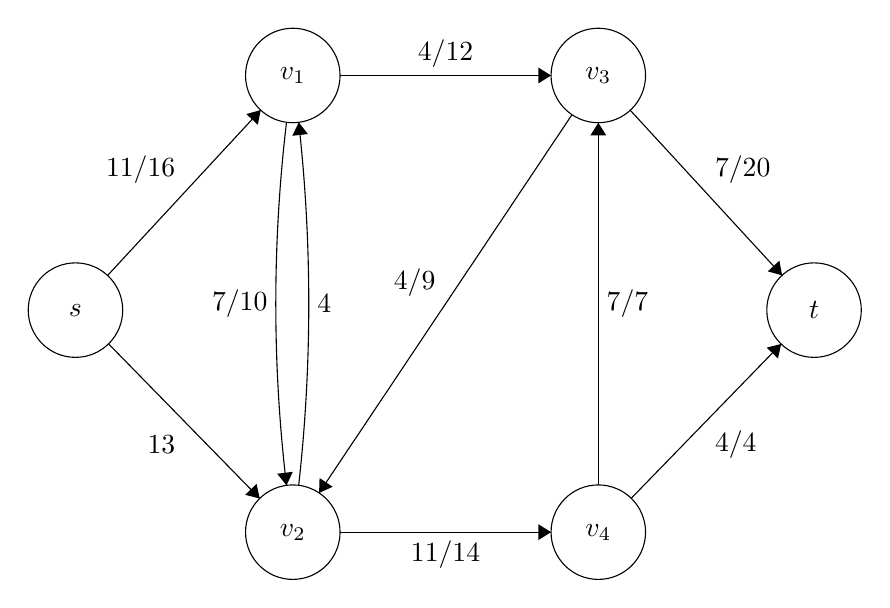
\begin{tikzpicture}[scale=0.2]
            \tikzstyle{every node}+=[inner sep=0pt]
            \draw [black] (5.1,-26) circle (3);
            \draw (5.1,-26) node {$s$};
            \draw [black] (18.9,-11.1) circle (3);
            \draw (18.9,-11.1) node {$v_1$};
            \draw [black] (18.9,-40.1) circle (3);
            \draw (18.9,-40.1) node {$v_2$};
            \draw [black] (38.3,-11.1) circle (3);
            \draw (38.3,-11.1) node {$v_3$};
            \draw [black] (38.3,-40.1) circle (3);
            \draw (38.3,-40.1) node {$v_4$};
            \draw [black] (52,-26) circle (3);
            \draw (52,-26) node {$t$};
            \draw [black] (7.14,-23.8) -- (16.86,-13.3);
            \fill [black] (16.86,-13.3) -- (15.95,-13.55) -- (16.68,-14.23);
            \draw (11.47,-17.09) node [left] {$11/16$};
            \draw [black] (21.9,-11.1) -- (35.3,-11.1);
            \fill [black] (35.3,-11.1) -- (34.5,-10.6) -- (34.5,-11.6);
            \draw (28.6,-10.6) node [above] {$4/12$};
            \draw [black] (40.33,-13.31) -- (49.97,-23.79);
            \fill [black] (49.97,-23.79) -- (49.8,-22.86) -- (49.06,-23.54);
            \draw (45.68,-17.09) node [right] {$7/20$};
            \draw [black] (40.39,-37.95) -- (49.91,-28.15);
            \fill [black] (49.91,-28.15) -- (48.99,-28.38) -- (49.71,-29.07);
            \draw (45.68,-34.52) node [right] {$4/4$};
            \draw [black] (38.3,-37.1) -- (38.3,-14.1);
            \fill [black] (38.3,-14.1) -- (37.8,-14.9) -- (38.8,-14.9);
            \draw (38.8,-25.6) node [right] {$7/7$};
            \draw [black] (36.63,-13.59) -- (20.57,-37.61);
            \fill [black] (20.57,-37.61) -- (21.43,-37.22) -- (20.6,-36.66);
            \draw (27.99,-24.26) node [left] {$4/9$};
            \draw [black] (21.9,-40.1) -- (35.3,-40.1);
            \fill [black] (35.3,-40.1) -- (34.5,-39.6) -- (34.5,-40.6);
            \draw (28.6,-40.6) node [below] {$11/14$};
            \draw [black] (18.501,-37.127) arc (-173.22938:-186.77062:97.772);
            \fill [black] (18.5,-37.13) -- (18.9,-36.27) -- (17.91,-36.39);
            \draw (17.32,-25.6) node [left] {$7/10$};
            \draw [black] (19.275,-14.076) arc (6.36043:-6.36043:104.021);
            \fill [black] (19.28,-14.08) -- (18.87,-14.93) -- (19.86,-14.82);
            \draw (20.42,-25.6) node [right] {$4$};
            \draw [black] (7.2,-28.14) -- (16.8,-37.96);
            \fill [black] (16.8,-37.96) -- (16.6,-37.03) -- (15.88,-37.73);
            \draw (11.47,-34.52) node [left] {$13$};
        \end{tikzpicture}
    \end{center}
    We continue picking augmenting paths and pushing flow through it
    until we result in a maximum flow graph, which looks as follows.
        \begin{center}
        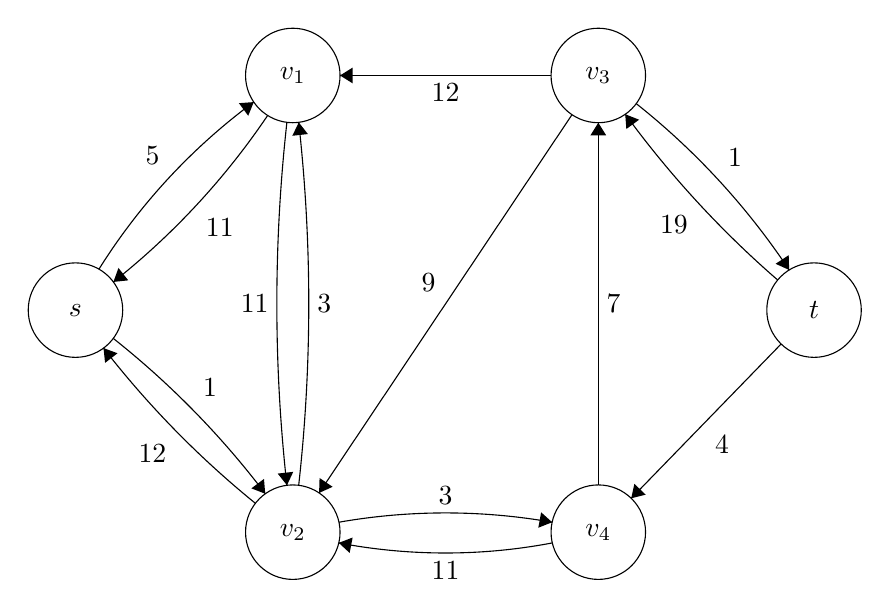
\begin{tikzpicture}[scale=0.2]
            \tikzstyle{every node}+=[inner sep=0pt]
            \draw [black] (5.1,-26) circle (3);
            \draw (5.1,-26) node {$s$};
            \draw [black] (18.9,-11.1) circle (3);
            \draw (18.9,-11.1) node {$v_1$};
            \draw [black] (18.9,-40.1) circle (3);
            \draw (18.9,-40.1) node {$v_2$};
            \draw [black] (38.3,-11.1) circle (3);
            \draw (38.3,-11.1) node {$v_3$};
            \draw [black] (38.3,-40.1) circle (3);
            \draw (38.3,-40.1) node {$v_4$};
            \draw [black] (52,-26) circle (3);
            \draw (52,-26) node {$t$};
            \draw [black] (6.592,-23.398) arc (147.95262:126.43724:38.744);
            \fill [black] (16.42,-12.79) -- (15.48,-12.86) -- (16.07,-13.66);
            \draw (10.47,-16.17) node [left] {$5$};
            \draw [black] (40.709,-12.887) arc (51.55917:33.63562:46.056);
            \fill [black] (50.42,-23.45) -- (50.39,-22.51) -- (49.56,-23.06);
            \draw (46.51,-16.33) node [right] {$1$};
            \draw [black] (38.3,-37.1) -- (38.3,-14.1);
            \fill [black] (38.3,-14.1) -- (37.8,-14.9) -- (38.8,-14.9);
            \draw (38.8,-25.6) node [right] {$7$};
            \draw [black] (36.63,-13.59) -- (20.57,-37.61);
            \fill [black] (20.57,-37.61) -- (21.43,-37.22) -- (20.6,-36.66);
            \draw (27.99,-24.26) node [left] {$9$};
            \draw [black] (21.832,-39.468) arc (99.96226:80.03774:39.122);
            \fill [black] (35.37,-39.47) -- (34.67,-38.84) -- (34.49,-39.82);
            \draw (28.6,-38.38) node [above] {$3$};
            \draw [black] (18.525,-37.124) arc (-173.65023:-186.34977:104.194);
            \fill [black] (18.53,-37.12) -- (18.93,-36.27) -- (17.94,-36.38);
            \draw (17.39,-25.6) node [left] {$11$};
            \draw [black] (19.275,-14.076) arc (6.36043:-6.36043:104.021);
            \fill [black] (19.28,-14.08) -- (18.87,-14.93) -- (19.86,-14.82);
            \draw (20.42,-25.6) node [right] {$3$};
            \draw [black] (7.501,-27.797) arc (51.61666:37.15122:54.809);
            \fill [black] (17.15,-37.66) -- (17.07,-36.72) -- (16.27,-37.32);
            \draw (13.17,-30.95) node [right] {$1$};
            \draw [black] (17.303,-13.639) arc (-33.99963:-51.61051:47.076);
            \fill [black] (7.51,-24.21) -- (8.45,-24.11) -- (7.83,-23.32);
            \draw (13.35,-20.77) node [right] {$11$};
            \draw [black] (35.3,-11.1) -- (21.9,-11.1);
            \fill [black] (21.9,-11.1) -- (22.7,-11.6) -- (22.7,-10.6);
            \draw (28.6,-11.6) node [below] {$12$};
            \draw [black] (35.38,-40.783) arc (-79.20925:-100.79075:36.212);
            \fill [black] (21.82,-40.78) -- (22.51,-41.42) -- (22.7,-40.44);
            \draw (28.6,-41.92) node [below] {$11$};
            \draw [black] (49.91,-28.15) -- (40.39,-37.95);
            \fill [black] (40.39,-37.95) -- (41.31,-37.72) -- (40.59,-37.03);
            \draw (45.68,-34.52) node [right] {$4$};
            \draw [black] (16.525,-38.268) arc (-129.07049:-142.16163:60.477);
            \fill [black] (6.88,-28.41) -- (6.98,-29.35) -- (7.77,-28.74);
            \draw (10.9,-35.09) node [left] {$12$};
            \draw [black] (49.689,-24.087) arc (-130.96495:-143.84027:63.756);
            \fill [black] (40.01,-13.56) -- (40.08,-14.5) -- (40.89,-13.91);
            \draw (44.02,-20.56) node [left] {$19$};
        \end{tikzpicture}
    \end{center}
\end{example}

The running time of this algorithm strongly depends on how
augmenting paths are determined.
If they are chosen poorly, the value of flow \emph{increases} with
each iteration but possibly \emph{too slowly}.
In extreme cases, it might \emph{never terminate} or even
\emph{not converge} to the value of maximum flow
(if capacities are irrational).
However, it practise capacities are typically integers
(which will always terminate).
If all capacities are small, then this is an efficient algorithm.

% todo
